% answers.tex —— 1977 年·江苏连云港市初试卷 · 参考答案与详细解析片段
% 由 tools/generate_projects.py 依来源总账自 1977/1977_数学真题_江苏连云港市初试_试题.md + 1977/1977_数学真题_江苏连云港市初试_解析正文.md + 1977/1977_数学真题_江苏连云港市初试_答案要点.md 生成，勿手改（改源 MD 后重跑）


\begin{gktip}
固定源为纯题面扫描，未附答案，下文逐题独立推导并复算。第 4 题保留原卷「求极根」这一疑似排印讹误的标题，按题干实际的极限记号求解；附加题 9 的解析接在第 8 题之后。
\end{gktip}

\begin{answer}
\gksolhead{1}{}

\textbf{题目}：

填充（每空 2 分）：

（1） 把指数式 $3^2=9$ 改写成对数式 $\underline{\hspace{3em}}$。

（2） 写出下列数列的通项公式：

① $2,4,6,8,10,\cdots\cdots$，$a_n=\underline{\hspace{2em}}$；

② $-1,1,-1,1,\cdots\cdots$，$a_n=\underline{\hspace{2em}}$；

（3） 以点 $(0,0)$ 为圆心，以 $4$ 为半径的圆的方程是 $\underline{\hspace{3em}}$。

\Needspace{4\baselineskip}
\textbf{解析}

\gksubpart{（1）}

\Needspace{5\baselineskip}
指数式 $3^2=9$ 中，底数 $3$、指数 $2$、幂 $9$，按对数定义改写为

\nopagebreak[4]
\[
\log_3 9=2.
\]

\gksubpart{（2）}

\Needspace{5\baselineskip}
① 数列 $2,4,6,8,10,\cdots\cdots$ 是首项为 $2$、公差为 $2$ 的等差数列，通项公式为

\nopagebreak[4]
\[
a_n=2n.
\]

\Needspace{5\baselineskip}
② 数列 $-1,1,-1,1,\cdots\cdots$ 各项正负交替，且奇数项为 $-1$、偶数项为 $1$，通项公式为

\nopagebreak[4]
\[
a_n=(-1)^n.
\]

\gksubpart{（3）}

\Needspace{5\baselineskip}
以 $(0,0)$ 为圆心、$4$ 为半径的圆的方程为

\nopagebreak[4]
\[
x^2+y^2=16.
\]

\gkanswer{答案（1）：$\log_3 9=2$。}

\gkanswer{答案（2）：① $a_n=2n$；② $a_n=(-1)^n$。}

\gkanswer{答案（3）：$x^2+y^2=16$。}

\end{answer}
\begin{answer}
\gksolhead{2}{}

\textbf{题目}：

计算：

（1） $1^{0.123}\times\left(\dfrac32\right)^{-3}\div\left(-\dfrac9{10}\right)^0$；

（2） $\log_{27}81-\lg100$；

（3） $\dfrac{\sqrt[3]{x^{\frac72}\sqrt{x^{-1}}}}{\sqrt{\sqrt[3]{x^{-7}}\sqrt[5]{x^{13}}}}$；

（4） $\dfrac{\left(\sin22^\circ30'+\cos22^\circ30'\right)^2}{2\cos0^\circ-2\sin15^\circ\cos15^\circ+\sin270^\circ}$。

\Needspace{4\baselineskip}
\textbf{解析}

\gksubpart{（1）}

\nopagebreak[4]
\[
1^{0.123}\times\left(\frac32\right)^{-3}\div\left(-\frac9{10}\right)^0
=1\times\left(\frac23\right)^3\times1
=\frac{8}{27}.
\]

\gksubpart{（2）}

\Needspace{5\baselineskip}
因为 $27=3^3$、$81=3^4$，所以 $\log_{27}81=\dfrac43$；又 $\lg100=2$，故

\nopagebreak[4]
\[
\log_{27}81-\lg100=\frac43-2=-\frac23.
\]

\gksubpart{（3）}

\Needspace{5\baselineskip}
先化简分子：

\nopagebreak[4]
\[
\sqrt[3]{x^{\frac72}\sqrt{x^{-1}}}
=\sqrt[3]{x^{\frac72-\frac12}}
=\sqrt[3]{x^{3}}=x.
\]

\Needspace{5\baselineskip}
再化简分母：

\nopagebreak[4]
\[
\sqrt{\sqrt[3]{x^{-7}}\sqrt[5]{x^{13}}}
=\sqrt{x^{-\frac73+\frac{13}5}}
=\sqrt{x^{\frac{4}{15}}}
=x^{\frac2{15}}.
\]

\Needspace{5\baselineskip}
所以（$x>0$）

\nopagebreak[4]
\[
\frac{\sqrt[3]{x^{\frac72}\sqrt{x^{-1}}}}{\sqrt{\sqrt[3]{x^{-7}}\sqrt[5]{x^{13}}}}
=\frac{x}{x^{\frac2{15}}}
=x^{\frac{13}{15}}.
\]

\gksubpart{（4）}

\Needspace{5\baselineskip}
利用 $(\sin\theta+\cos\theta)^2=1+\sin2\theta$，分子

\nopagebreak[4]
\[
(\sin22^\circ30'+\cos22^\circ30')^2=1+\sin45^\circ=1+\frac{\sqrt2}2.
\]

\Needspace{5\baselineskip}
分母

\nopagebreak[4]
\[
2\cos0^\circ-2\sin15^\circ\cos15^\circ+\sin270^\circ
=2-\sin30^\circ-1
=2-\frac12-1=\frac12.
\]

\Needspace{5\baselineskip}
所以原式

\nopagebreak[4]
\[
=\frac{1+\dfrac{\sqrt2}2}{\dfrac12}=2+\sqrt2.
\]

\gkanswer{答案（1）：$\dfrac{8}{27}$。}

\gkanswer{答案（2）：$-\dfrac23$。}

\gkanswer{答案（3）：$x^{\frac{13}{15}}$（$x>0$）。}

\gkanswer{答案（4）：$2+\sqrt2$。}

\end{answer}
\begin{answer}
\gksolhead{3}{}

\textbf{题目}：

对于下列函数，写出自变量 $x$ 的取值范围：

（1） $y=\dfrac{6x-1}{2x-1}$；

（2） $y=\sqrt{x}+\sqrt{-x}$；

（3） $y=\sqrt{\lg\dfrac12(x+1)}$。

\Needspace{4\baselineskip}
\textbf{解析}

\gksubpart{（1）}

$y=\dfrac{6x-1}{2x-1}$ 要求分母不为零，即 $2x-1\ne0$，故 $x\in\mathbf R$ 且 $x\ne\dfrac12$。

\gksubpart{（2）}

$y=\sqrt{x}+\sqrt{-x}$ 要求 $x\ge0$ 且 $-x\ge0$，两者同时成立只有 $x=0$。

\gksubpart{（3）}

\Needspace{5\baselineskip}
$y=\sqrt{\lg\dfrac12(x+1)}$ 要求根号内非负，即

\nopagebreak[4]
\[
\lg\left[\frac12(x+1)\right]\ge0
\quad\Longrightarrow\quad
\frac12(x+1)\ge1
\quad\Longrightarrow\quad
x\ge1.
\]

\gkanswer{答案（1）：$x\in\mathbf R$ 且 $x\ne\dfrac12$。}

\gkanswer{答案（2）：$x=0$。}

\gkanswer{答案（3）：$x\ge1$。}

\end{answer}
\begin{answer}
\gksolhead{4}{}

\textbf{题目}：

\Needspace{5\baselineskip}
求极根

\nopagebreak[4]
\[
\lim_{n\to\infty}\left[\frac{1+3+5+\cdots\cdots+(2n-1)}{n+2}-n\right].
\]

\begin{gktip}
\textbf{源注}：原卷本大题标题印作「求极根」，据后接极限记号 $\lim\limits_{n\to\infty}[\cdots]$ 判断，当为「求极限」之排印讹误；本文按原卷字面保留，解析按「求极限」处理。
\end{gktip}

\Needspace{4\baselineskip}
\textbf{解析}

\Needspace{5\baselineskip}
由 $1+3+5+\cdots\cdots+(2n-1)=n^2$（前 $n$ 个奇数之和），原式为

\nopagebreak[4]
\[
\lim_{n\to\infty}\left[\frac{n^2}{n+2}-n\right]
=\lim_{n\to\infty}\frac{n^2-n(n+2)}{n+2}
=\lim_{n\to\infty}\frac{-2n}{n+2}.
\]

\Needspace{5\baselineskip}
分子分母同除以 $n$：

\nopagebreak[4]
\[
\lim_{n\to\infty}\frac{-2}{1+\dfrac2n}=-2.
\]

\gkanswer{答案：$-2$。}

\end{answer}
\begin{answer}
\gksolhead{5}{}

\textbf{题目}：

（1） $k$ 为何值时，方程 $x^2-2kx+3=0$ 有一个根是 $-2$？

（2） 试判别一元二次方程 $ax^2+(a-b)x-(a+b)=0$ 的根的情况。

\Needspace{4\baselineskip}
\textbf{解析}

\gksubpart{（1）}

\Needspace{5\baselineskip}
$x=-2$ 是方程 $x^2-2kx+3=0$ 的根，代入：

\nopagebreak[4]
\[
4+4k+3=0\quad\Longrightarrow\quad k=-\frac74.
\]

\gksubpart{（2）}

\Needspace{5\baselineskip}
先看 $a\ne0$ 的情形。此时方程为一元二次方程，判别式

\nopagebreak[4]
\[
\Delta=(a-b)^2+4a(a+b)=a^2-2ab+b^2+4a^2+4ab=5a^2+2ab+b^2=(a+b)^2+4a^2.
\]

因为 $a\ne0$，故 $4a^2>0$，而 $(a+b)^2\ge0$，所以 $\Delta>0$ 恒成立，方程有两个不相等的实数根。

\Needspace{5\baselineskip}
再看 $a=0$ 的情形。方程退化为

\nopagebreak[4]
\[
(0-b)x-(0+b)=-bx-b=-b(x+1)=0.
\]

若 $b\ne0$，得唯一实根 $x=-1$；若 $a=b=0$，方程恒为 $0=0$，对任意 $x$ 都成立。

\gkanswer{答案（1）：$k=-\dfrac74$。}

\gkanswer{答案（2）：当 $a\ne0$ 时，判别式 $\Delta=(a+b)^2+4a^2>0$ 恒成立，方程有两个不相等的实数根；当 $a=0$、$b\ne0$ 时，方程退化为一次方程，有唯一实根 $x=-1$；当 $a=b=0$ 时，方程对任意 $x$ 都成立。}

\end{answer}
\begin{answer}
\gksolhead{6}{}

\textbf{题目}：

\Needspace{5\baselineskip}
已知椭圆

\nopagebreak[4]
\[
\frac{x^2}{5^2}+\frac{y^2}{3^2}=1,
\]

（1） 求此椭圆的长轴的长、离心率、焦点坐标和准线方程；

（2） 如图过椭圆的一个焦点 $F$，作 $FA$ 平行于 $Y$ 轴交椭圆的上半部于 $A$ 点，求 $A$ 点的坐标；
\nopagebreak[4]
\begin{center}% 1977 年江苏连云港市初试卷第 6 题：椭圆 x²/5²+y²/3²=1，
% 焦点 F 在正 X 轴上，过 F 作 FA 平行于 Y 轴交椭圆上半部于 A，标出三角形 AOF（按源卷第 2 页布局）
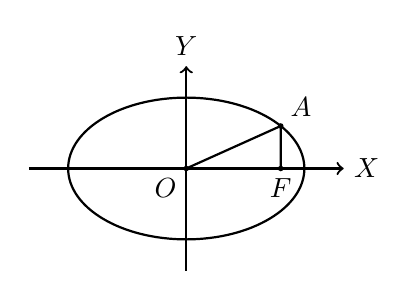
\begin{tikzpicture}[scale=1]
  \draw[thick,->] (-2,0) -- (2,0) node[right] {$X$};
  \draw[thick,->] (0,-1.3) -- (0,1.3) node[above] {$Y$};
  \draw[thick] (0,0) ellipse (1.5 and 0.9);
  \coordinate (O) at (0,0);
  \coordinate (F) at (1.2,0);
  \coordinate (A) at (1.2,0.54);
  \draw[thick] (O) -- (A) -- (F);
  \fill (O) circle (1pt) node[below left] {$O$};
  \fill (F) circle (1pt) node[below] {$F$};
  \fill (A) circle (1pt) node[above right] {$A$};
\end{tikzpicture}
\end{center}
\nopagebreak[4]
（3） 求 $\triangle AOF$ 的面积。

\Needspace{4\baselineskip}
\textbf{解析}

\gksubpart{（1）}

\Needspace{5\baselineskip}
椭圆 $\dfrac{x^2}{5^2}+\dfrac{y^2}{3^2}=1$ 中 $a=5$、$b=3$，故

\nopagebreak[4]
\[
c=\sqrt{a^2-b^2}=\sqrt{25-9}=4.
\]

长轴长 $2a=10$；离心率 $e=\dfrac ca=\dfrac45$；焦点坐标 $(\pm4,0)$；准线方程 $x=\pm\dfrac{a^2}c=\pm\dfrac{25}4$。

\gksubpart{（2）}

\Needspace{5\baselineskip}
取右焦点 $F(4,0)$。$FA$ 平行于 $Y$ 轴，故 $A$ 的横坐标为 $4$。代入椭圆方程：

\nopagebreak[4]
\[
\frac{4^2}{25}+\frac{y^2}9=1
\quad\Longrightarrow\quad
\frac{y^2}9=1-\frac{16}{25}=\frac9{25}
\quad\Longrightarrow\quad
y^2=\frac{81}{25}.
\]

取上半部正值 $y=\dfrac95$，故 $A\left(4,\dfrac95\right)$。

\gksubpart{（3）}

\Needspace{5\baselineskip}
$\triangle AOF$ 以 $OF$ 为底、$A$ 到 $OF$（即 $X$ 轴）的距离为高。$OF=4$，高为 $A$ 的纵坐标 $\dfrac95$，故

\nopagebreak[4]
\[
S_{\triangle AOF}=\frac12\times4\times\frac95=\frac{18}5.
\]

\gkanswer{答案（1）：长轴长 $10$，离心率 $e=\dfrac45$，焦点坐标 $(\pm4,0)$，准线方程 $x=\pm\dfrac{25}{4}$。}

\gkanswer{答案（2）：$A\left(4,\dfrac95\right)$。}

\gkanswer{答案（3）：$\dfrac{18}{5}$。}

\end{answer}
\begin{answer}
\gksolhead{7}{}

\textbf{题目}：

如图：把小矩形 $ABCD$ 扩充为大矩形 $AEFG$，并使 $BE+EF+FG+GD=22$，已知小矩形的宽 $AB=2$，小矩形的周长为 $12$，问 $BE$ 为何值时扩充部分的面积最大？最大面积是多少？（扩充部分为图中阴影部分）
\nopagebreak[4]
\begin{center}% 1977 年江苏连云港市初试卷第 7 题：小矩形 ABCD 扩充为大矩形 AEFG，
% 阴影（斜线填充）部分为扩充增加的面积（按源卷第 2—3 页「第七题图」布局）
\begin{tikzpicture}[scale=1]
  \coordinate (A) at (0,2.8);
  \coordinate (D) at (1.6,2.8);
  \coordinate (G) at (2.8,2.8);
  \coordinate (B) at (0,2.0);
  \coordinate (C) at (1.6,2.0);
  \coordinate (E) at (0,0);
  \coordinate (F) at (2.8,0);
  \path[pattern=north east lines, even odd rule] (E) rectangle (G) (B) rectangle (D);
  \draw[thick] (A) -- (G) -- (F) -- (E) -- cycle;
  \draw[thick] (A) -- (D) -- (C) -- (B) -- cycle;
  \fill (A) circle (1.2pt) node[above left] {$A$};
  \fill (D) circle (1.2pt) node[above] {$D$};
  \fill (G) circle (1.2pt) node[above right] {$G$};
  \fill (B) circle (1.2pt) node[left] {$B$};
  \fill (C) circle (1.2pt) node[above right] {$C$};
  \fill (E) circle (1.2pt) node[below left] {$E$};
  \fill (F) circle (1.2pt) node[below right] {$F$};
\end{tikzpicture}
\end{center}
\nopagebreak[4]
\Needspace{4\baselineskip}
\textbf{解析}

设小矩形 $ABCD$ 中 $AB=2$（竖边）。小矩形周长为 $12$，即 $2(AB+AD)=12$，故 $AD=4$（横边）。

设 $BE=t$（左边向下扩充的长度），$DG=s$（上边向右扩充的长度）。大矩形 $AEFG$ 的左边 $AE=AB+BE=2+t$，上边 $AG=AD+DG=4+s$；由矩形对边相等，$FG=AE=2+t$，$EF=AG=4+s$。

\Needspace{5\baselineskip}
由 $BE+EF+FG+GD=22$：

\nopagebreak[4]
\[
t+(4+s)+(2+t)+s=22
\quad\Longrightarrow\quad
2t+2s+6=22
\quad\Longrightarrow\quad
t+s=8.
\]

\Needspace{5\baselineskip}
扩充部分（阴影）面积为大矩形减小矩形：

\nopagebreak[4]
\[
S(t)=(2+t)(4+s)-2\times4=(2+t)(4+s)-8.
\]

\Needspace{5\baselineskip}
代入 $s=8-t$：

\nopagebreak[4]
\[
S(t)=(2+t)(12-t)-8=24+10t-t^2-8=-t^2+10t+16.
\]

\Needspace{5\baselineskip}
对 $t$ 求导并令其为零：

\nopagebreak[4]
\[
S'(t)=-2t+10=0\quad\Longrightarrow\quad t=5.
\]

\Needspace{5\baselineskip}
由于 $S(t)$ 的二次项系数为负，$t=5$ 处取得最大值，且 $t=5$ 在有效范围 $0\le t\le8$ 内。代入得

\nopagebreak[4]
\[
S(5)=-25+50+16=41.
\]

故 $BE=5$ 时扩充部分面积最大，最大面积为 $41$。

\begin{gktip}
\textbf{核验}：此时 $s=8-5=3$，大矩形边长 $AE=7$、$AG=7$，恰为正方形，面积 $49$；小矩形面积 $8$；扩充部分 $49-8=41$，与上式一致。
\end{gktip}

\gkanswer{答案：$BE=5$ 时扩充部分的面积最大，最大面积为 $41$。}

\end{answer}
\begin{answer}
\gksolhead{8}{}

\textbf{题目}：

已知 $AD$ 是 $\odot O$ 的弦，且 $AD=8$，半径 $OH\perp AD$，交 $AD$ 于 $B$ 点，且 $HB=2$，又 $AC$ 是圆的直径，试求 $BC$ 的长。
\nopagebreak[4]
\begin{center}% 1977 年江苏连云港市初试卷第 8 题：⊙O 中弦 AD、直径 AC，
% 半径 OH⊥AD 交 AD 于 B，求 BC 的长（按源卷第 3 页「第八题」布局，AB=BD=4、OB=3、半径=5 等比例缩放）
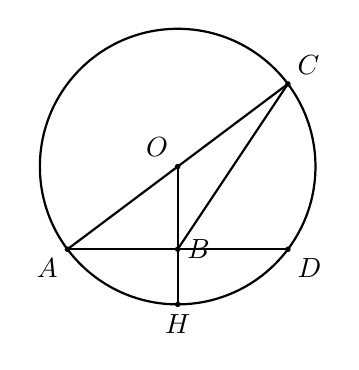
\begin{tikzpicture}[scale=1]
  \coordinate (O) at (0,0);
  \coordinate (A) at (-1.4,-1.05);
  \coordinate (D) at (1.4,-1.05);
  \coordinate (H) at (0,-1.75);
  \coordinate (C) at (1.4,1.05);
  \coordinate (B) at (0,-1.05);
  \draw[thick] (O) circle (1.75);
  \draw[thick] (A) -- (D);
  \draw[thick] (A) -- (C);
  \draw[thick] (O) -- (H);
  \draw[thick] (B) -- (C);
  \fill (O) circle (1pt) node[above left] {$O$};
  \fill (A) circle (1pt) node[below left] {$A$};
  \fill (D) circle (1pt) node[below right] {$D$};
  \fill (H) circle (1pt) node[below] {$H$};
  \fill (C) circle (1pt) node[above right] {$C$};
  \fill (B) circle (1pt) node[right] {$B$};
\end{tikzpicture}
\end{center}
\nopagebreak[4]
\textbf{附加题 9．} 如图 $A$ 是双曲线 $x^2-y^2=1$ 上的一点，$A$ 点处的法线交坐标轴于 $B$、$C$ 两点，若 $|BC|=42$，试求 $|OA|$。

\begin{gktip}
\textbf{提示}：设 $A(x_0,y_0)$，先求出法线斜率，次写出方程，找出 $B$、$C$ 坐标，再用距离公式求出 $A$ 点坐标。
\end{gktip}
\nopagebreak[4]
\begin{center}% 1977 年江苏连云港市初试卷附加题（第 9 题）：双曲线 x²-y²=1 上一点 A，
% A 点处法线交坐标轴于 B（Y 轴）、C（X 轴），B、A、C 三点共线（按源卷第 3 页「附加题」布局，取样例点示意）
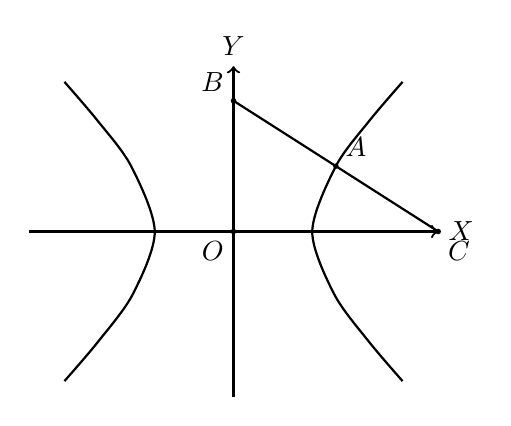
\begin{tikzpicture}[scale=1]
  \draw[thick,->] (-2.6,0) -- (2.6,0) node[right] {$X$};
  \draw[thick,->] (0,-2.1) -- (0,2.1) node[above] {$Y$};
  \draw[thick] plot[smooth] coordinates {(2.147,-1.9) (1.720,-1.4) (1.281,-0.8) (1,0) (1.3,0.83) (1.720,1.4) (2.147,1.9)};
  \draw[thick] plot[smooth] coordinates {(-2.147,-1.9) (-1.720,-1.4) (-1.281,-0.8) (-1,0) (-1.3,0.83) (-1.720,1.4) (-2.147,1.9)};
  \coordinate (O) at (0,0);
  \coordinate (B) at (0,1.66);
  \coordinate (A) at (1.3,0.83);
  \coordinate (C) at (2.6,0);
  \draw[thick] (B) -- (C);
  \fill (O) circle (1pt) node[below left] {$O$};
  \fill (B) circle (1pt) node[above left] {$B$};
  \fill (A) circle (1pt) node[above right] {$A$};
  \fill (C) circle (1pt) node[below right] {$C$};
\end{tikzpicture}
\end{center}
\nopagebreak[4]
\Needspace{4\baselineskip}
\textbf{解析}

因为半径 $OH\perp AD$ 且 $B$ 为垂足，所以 $OH$ 平分弦 $AD$，即 $AB=BD=\dfrac12AD=4$。

\Needspace{5\baselineskip}
设圆的半径为 $r$，则 $OH=r$，$OB=OH-HB=r-2$。在直角三角形 $OBD$ 中：

\nopagebreak[4]
\[
OB^2+BD^2=OD^2
\quad\Longrightarrow\quad
(r-2)^2+4^2=r^2.
\]

\Needspace{5\baselineskip}
展开：

\nopagebreak[4]
\[
r^2-4r+4+16=r^2
\quad\Longrightarrow\quad
-4r+20=0
\quad\Longrightarrow\quad
r=5.
\]

故 $OB=3$。以 $B$ 为原点、$AD$ 所在直线为横轴建立坐标系：$A(-4,0)$，$D(4,0)$，$O(0,3)$。

\Needspace{5\baselineskip}
因为 $AC$ 是直径，$O$ 为 $AC$ 中点，故

\nopagebreak[4]
\[
C=2O-A=(0-(-4),6-0)=(4,6).
\]

\Needspace{5\baselineskip}
于是

\nopagebreak[4]
\[
BC=\sqrt{(4-0)^2+(6-0)^2}=\sqrt{16+36}=\sqrt{52}=2\sqrt{13}.
\]

\textbf{附加题 9}

设 $A(x_0,y_0)$ 在双曲线 $x^2-y^2=1$ 上，即 $x_0^2-y_0^2=1$。

对 $x^2-y^2=1$ 两边关于 $x$ 求导：$2x-2yy'=0$，得切线斜率 $y'=\dfrac xy$，故 $A$ 处切线斜率为 $\dfrac{x_0}{y_0}$，法线斜率为 $-\dfrac{y_0}{x_0}$。

\Needspace{5\baselineskip}
法线方程：

\nopagebreak[4]
\[
y-y_0=-\frac{y_0}{x_0}(x-x_0).
\]

\Needspace{5\baselineskip}
令 $y=0$（求与 $X$ 轴交点 $C$）：

\nopagebreak[4]
\[
-y_0=-\frac{y_0}{x_0}(x-x_0)
\quad\Longrightarrow\quad
x_0=x-x_0
\quad\Longrightarrow\quad
x=2x_0,
\]

故 $C=(2x_0,0)$。

\Needspace{5\baselineskip}
令 $x=0$（求与 $Y$ 轴交点 $B$）：

\nopagebreak[4]
\[
y-y_0=-\frac{y_0}{x_0}(0-x_0)=y_0
\quad\Longrightarrow\quad
y=2y_0,
\]

故 $B=(0,2y_0)$。

\Needspace{5\baselineskip}
于是

\nopagebreak[4]
\[
|BC|^2=(2x_0)^2+(2y_0)^2=4(x_0^2+y_0^2)=4|OA|^2,
\]

\Needspace{5\baselineskip}
即 $|BC|=2|OA|$。已知 $|BC|=42$，故

\nopagebreak[4]
\[
|OA|=21.
\]

\gkanswer{答案：$BC=2\sqrt{13}$。}

\end{answer}